\chapter{Physics-based reconstruction using shell elements}
\label{chap10}
\begin{shortAbstract}
In the previous chapter, we proposed a co-rotational formulation for shell elements by extending a classical in-plane triangular finite element approach. This simple shell element can efficiently handle both membrane and offplane forces (bending and twist). The validity of our approach has been demonstrated though comparison with theoretical results. It was then applied it to a rather complex application: the simulation of intra-ocular lens implant deployment in a cataract surgery simulation. These preliminary results are very encouraging and show the potential of such models. Examples include the modelling of hollow anatomical structures (stomach, colon, etc.), the simulation of cardiac valve leaflets, and blood vessels. However, to model the deformation of complex anatomical structures using shell elements, the first step is to describe its surface with curved patches. In the next section, we propose to study how to approximate the surface of anatomical structures with (curved) shell elements. This work was the object of one publication \citep{Comas2010b}.
\end{shortAbstract}


\section{Techniques of mesh simplification}

\subsection{Introduction: our motivation}

Our idea is the following: while many flat triangles are required to describe highly curved surfaces, fewer triangular shell elements are needed to describe a given geometry with the same precision since they can be curved. Our goal is to create a mesh featuring the optimal number of shell elements while staying as close as possible to our targeted geometry. Literature about volumic mesh generation algorithms is fairly dense. However, there are only a few that are concerned about the generation of meshes over curved surfaces. One of the most widely used techniques for the creation of surface meshes is the plane to surface transformation method \citep{Zienkiewicz71}, mesh is first generated on a two-dimensional domain and then mapped onto the surface. If this method gives reasonably good meshes on smooth surfaces, the results are usually quite poor with more complex curved surfaces. The finite elements may be generated directly on the curved surfaces based on the advancing front technique \citep{Lo85,Lau96}. The main issue with this approach is that an analytical description of the geometry is needed, which is not the case in medical simulation. Another method consists of using an a priori error estimator to build an adaptive mesh generation \citep{Baumann97}. However, the tolerance of this indicator should be chosen depending on the desired accuracy of the finite element solution, and therefore requires some knowledge about the problem in order to choose an effective tolerance. \cite{Bechet02} start from an existing triangular mesh created with a CAD (computer-aided design) software and refine and smooth the mesh based on element quality and surface curvature. While all those methods allow their authors to get satisfactory meshes over curved surfaces according to their needs, they all make use of flat elements to mesh geometries and do not generate actual shells. 

In fact, it is interesting to note that this process of meshing a curved surface is similar to the reconstruction of the surface of objects in computer vision. Indeed, calculating curvature maps of 3D surfaces represented as digitised data (point clouds or triangulated meshes) has been extensively studied. One of the most common approach is to use continuous surface patches \citep{Kolb95,Douros02}. The surface is locally approximated by an analytic representation called surface patch, usually chosen to be an implicit surface. \cite{Tang99} presented an elegant and non noise-sensitive approach that infers sign and direction of principal curvatures directly from the input and the authors used this information for coherent surface and curve extraction from 3D data. 

However, we need to keep in mind that our situation is substantially different than all previously mentioned geometrical approaches as we want to model the deformation of the structure. In that regard, the curvature of the surface has a physical meaning: it represents the mid-surface of the shell. By keeping this in mind, we propose an approach to mesh a curved surface based on the same polynomial shape function \eqref{chap9:eq-deflection} used in our co-rotational shell FEM. 

%Simplification strategies may be grouped into two categories: local strategies that iteratively simplify the mesh by the repeated application of some local operator, and global strategies that are applied to the input mesh as a whole \citep{Cignoni97,Talton04}.
%
%\subsection{Local simplification strategies}
%
%Typically, they define some mesh operation $S$ that, when applied to a mesh $M$, acts on a small collection of its elements and produces a new mesh $\overline{M}$  with fewer elements. By repeated application of $S$, a mesh may be simplified arbitrarily. In order to determine the mesh elements to which $S$ should be applied on a given iteration, $S$ may be associated with an error function (or cost function) that measures the amount of error the operation will introduce into the approximation. By computing the error associated with every possible application of $S$ at a particular iteration, the algorithm can apply the one with minimal cost. This type of heuristic is quite reasonable for simplification problems, and in practice these methods work well.
%
%One nice property of local iterative algorithms is that they allow the user to specify the desired attributes of the target approximating mesh with a high degree of precision. For example, the user may allow the algorithm to run until the mesh contains $k$ faces, or until the error at a given vertex exceeds some threshold $\varepsilon$. 
%
%\subsubsection*{Vertex decimation.}
%The decimation algorithm, first proposed by \cite{Schroeder92}, is simple. Multiple passes are made over all vertices in the mesh. During a pass, each vertex is a candidate for removal and, if it meets the specified decimation criteria, the vertex and all triangles that use the vertex are deleted. The resulting hole in the mesh is patched by forming a local triangulation. The vertex removal process repeats, with possible adjustment of the decimation criteria, until some termination condition is met. 
%
%The error associated with a particular decimation typically depends on the classification of the vertex being decimated. For the general case of a manifold vertex $\lbrace i \rbrace$ not near a boundary, \citeauthor{Schroeder92} consider the set of planes formed by the adjacent triangles and compute a single approximating plane based on the area-weighted average of the triangle normals $\textbf{n}_k$, centers $x_k$, and areas $A_k$:
%%
%\begin{equation}
%\textbf{n} = \frac{\sum_k A_k\textbf{n}_k}{\sum_k A_k},  \hspace*{1cm} \widehat{\textbf{n}} = \frac{\textbf{n}}{\vert \textbf{n} \vert}, \hspace*{1cm}  x = \frac{\sum_k A_k\textbf{x}_k}{\sum_k A_k}
%\end{equation}
%
%Then they calculate the distance from vertex $\lbrace i \rbrace$ to this plane by  $\vert \widehat{\textbf{n}} \cdot (v_i - x) \vert$ and define this quantity to be the cost associated with the decimation. This metric ensures that vertices in smooth regions will be decimated before vertices that define sharp features. 
%
%In practice, simplification schemes based on vertex decimation excel at eliminating un-necessary geometry, such as is typically found in meshes generated by the marching cubes algorithm where large planar regions may be subdivided into many redundant triangles. 
%
%\subsubsection*{Edge contraction.}
%Edge contraction, originally proposed by \cite{Hoppe93}, is the most common simplification operation. An edge contraction operates on a single edge $\lbrace v_1,v_2 \rbrace$ and contracts that edge to a single vertex $\lbrace w \rbrace$, updating all edges previously incident on $\lbrace v_1 \rbrace$ and $\lbrace v_2 \rbrace$ to reference $\lbrace w \rbrace$. On a manifold mesh without boundary, each edge contraction will collapse precisely two faces (see \fig{chap10:fig-edgeCollapse}). Edge contractions can alter the topology of a mesh, since repeatedly contracting all the edges around a hole will eventually close it.
%%
%\begin{figure}
%\centering
%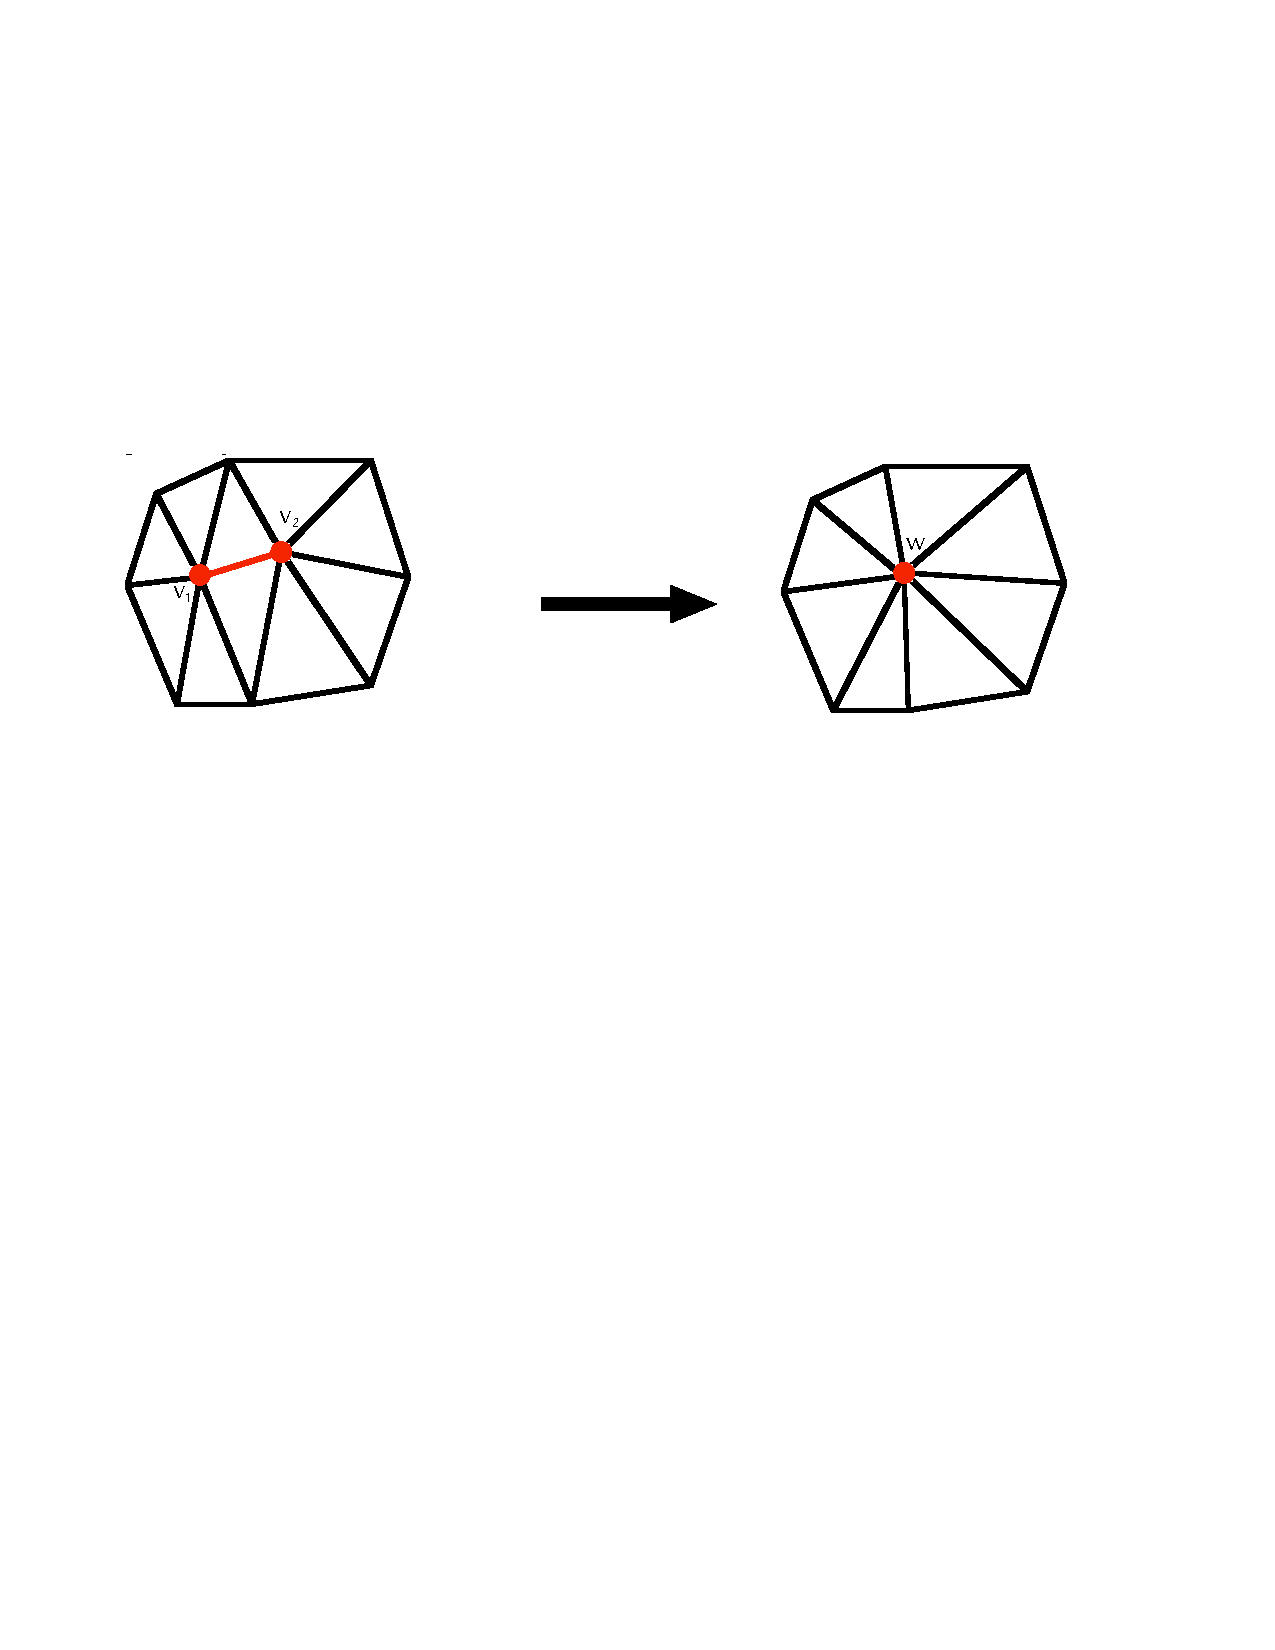
\includegraphics[height=3cm]{chapter10/edgeCollapse.pdf}
%\caption[The edge contraction operation]{The edge contraction operation. Image courtesy of \cite{Hoppe93}.}
%\label{chap10:fig-edgeCollapse}
%\end{figure}
%
%For a given contraction $\lbrace v_1,v_2 \rbrace \rightarrow \lbrace w \rbrace$, it is not immediately clear what value should be assigned to $v_h$, i.e. where the resulting vertex should be placed. Obvious choices such as $v_h = v_i$, $v_h = v_j$, or $v_h = (v_i + v_j)/2$ are convenient, but can easily be shown to be non-optimal. Rather than placing $v_h$ arbitrarily, it is better to consider the error function associated with the contraction operation and attempt to minimise its value over the space of possible vertex placements. Once the optimal target position has been computed for every possible contraction, the contraction with the smallest associated error can be selected and applied.
%
%\subsubsection*{Adaptative subdivision.}
%Coplanar or nearly coplanar faces are searched for in the mesh, merged into larger polygons, and then retriangulated into fewer faces than those originally required \citep{Dehaemer91,Hinker93}. Face merging is driven by a co-planarity test. 
%
%The basic adaptive subdivision method as presented by \cite{Schmitt86} is sketched in \fig{chap10:fig-adaptativeSubdivision}. (a) shows several data points produced by the sampling process and sketch (b) adds a trial polygon that approximates the surface represented by the sample points. A bilinear interpolation is performed over the surface of the approximating polygon to locate the point on the surface 'directly below' a sample data point. The distance (or error) between the surface and the data point is then calculated, as shown in (c), and is compared to the user specified tolerance. If any of the errors exceeds the tolerance value then the polygon is divided into four smaller polygons, as shown in (d), and the process is repeated recursively. 
%%
%\begin{figure}
%\centering
%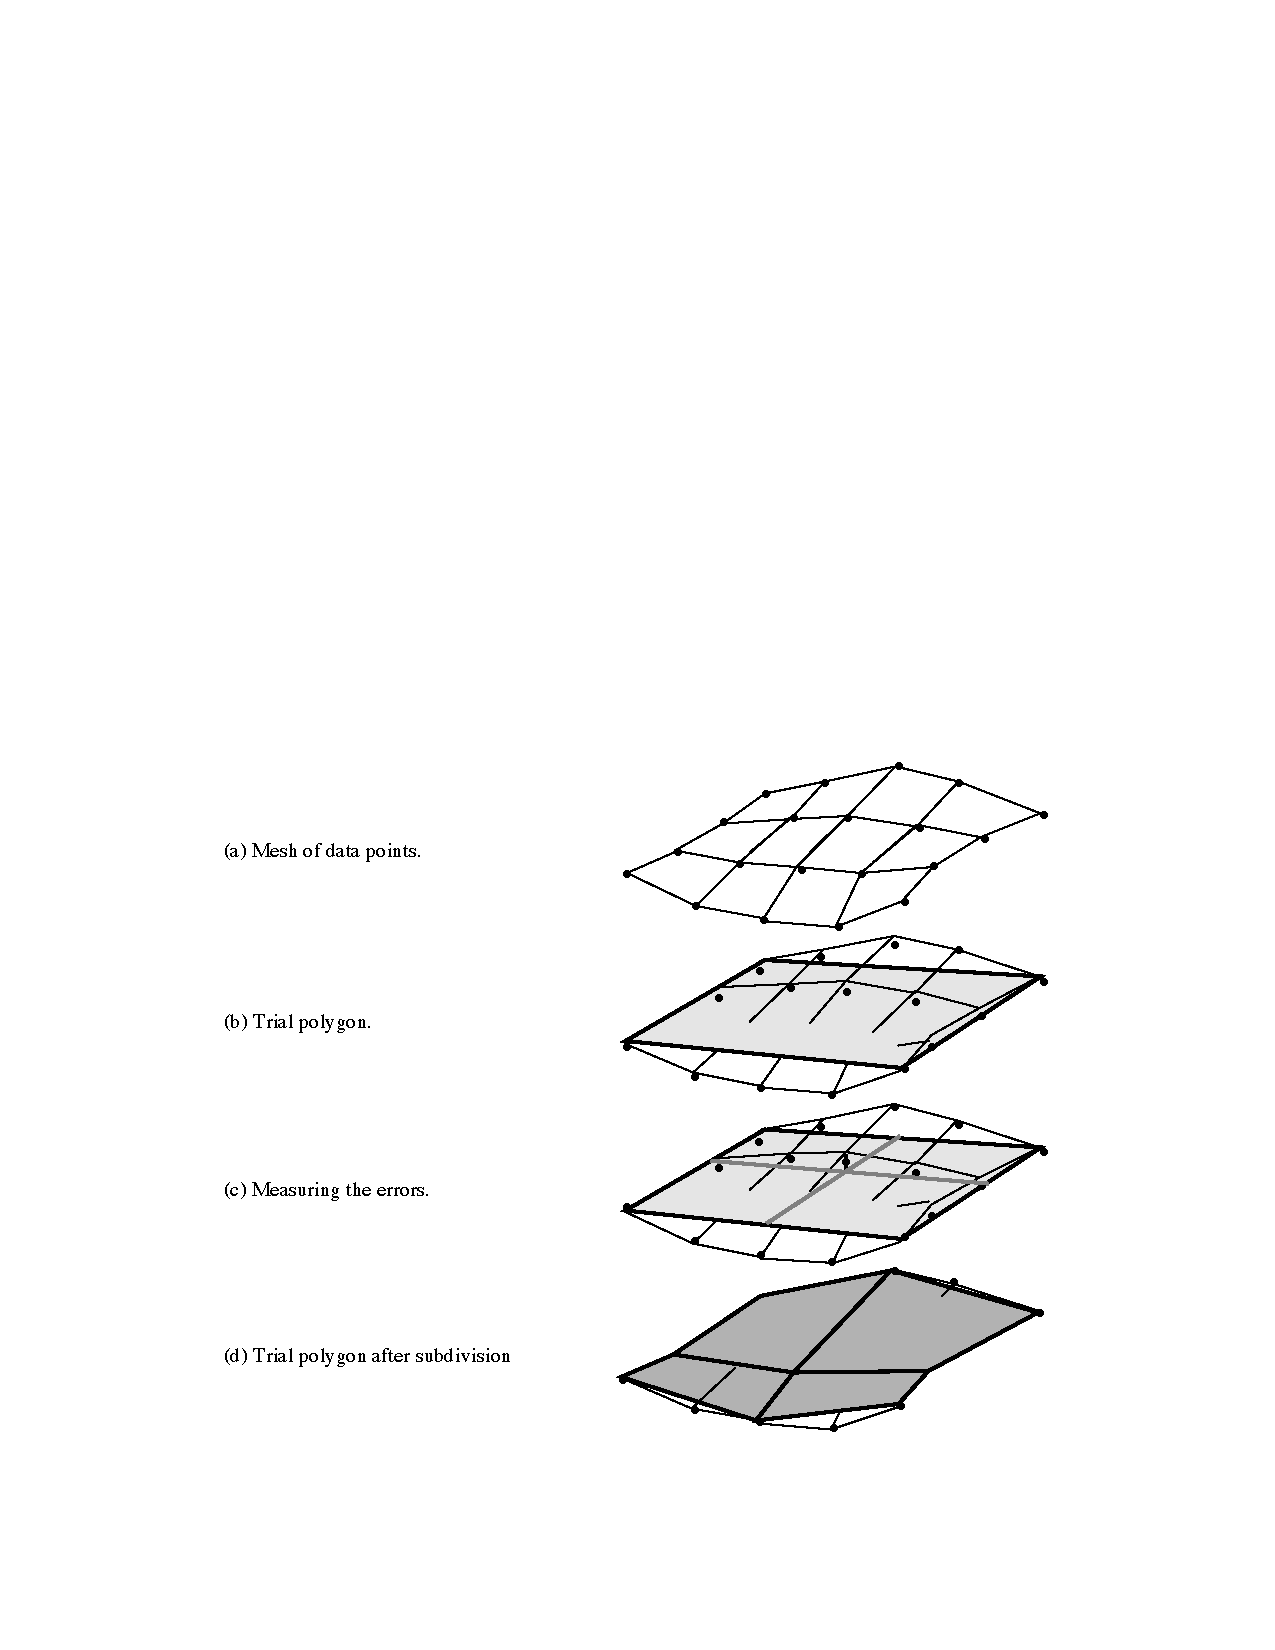
\includegraphics[width=13.5cm]{chapter10/adaptativeSubdivision.pdf}
%\caption[Surface-fitting polygons with adaptive subdivision]{Surface-fitting polygons with adaptive subdivision. Image courtesy of \cite{Schmitt86}.}
%\label{chap10:fig-adaptativeSubdivision}
%\end{figure}
%
%When the approximation to the data is within the specified tolerance, the recursion is terminated and the polygon is saved in a linked list. Upon completion of the subdivision algorithm, the resulting polygons are displayed for the user to judge the results. Generally, the user runs the program repeatedly while varying the maximum tolerance until the results are suitable.
%
%\subsubsection*{Polygon growth.}
%Another method proposed by \cite{Dehaemer91} to systematically generate surface-fitting polygons is to use a polygon growth technique (see \fig{chap10:fig-polygonGrowth}). First a seed polygon is selected from the original set of data, as in (a). Then a neighbouring polygon is selected and the two are combined into a larger trial polygon ((b) and (c)). If the trial polygon passes the accuracy metric, 10 additional neighbors are selected in an attempt at further growth, as in (d) through (g). When all attempts at further growth fail, the polygon is added to the list of polygons describing the reduced object, as shown in (h). A new seed polygon is selected and the process repeated. When there are no more polygons from which to choose a new seed, the process is terminated.
%%
%\begin{figure}
%\centering
%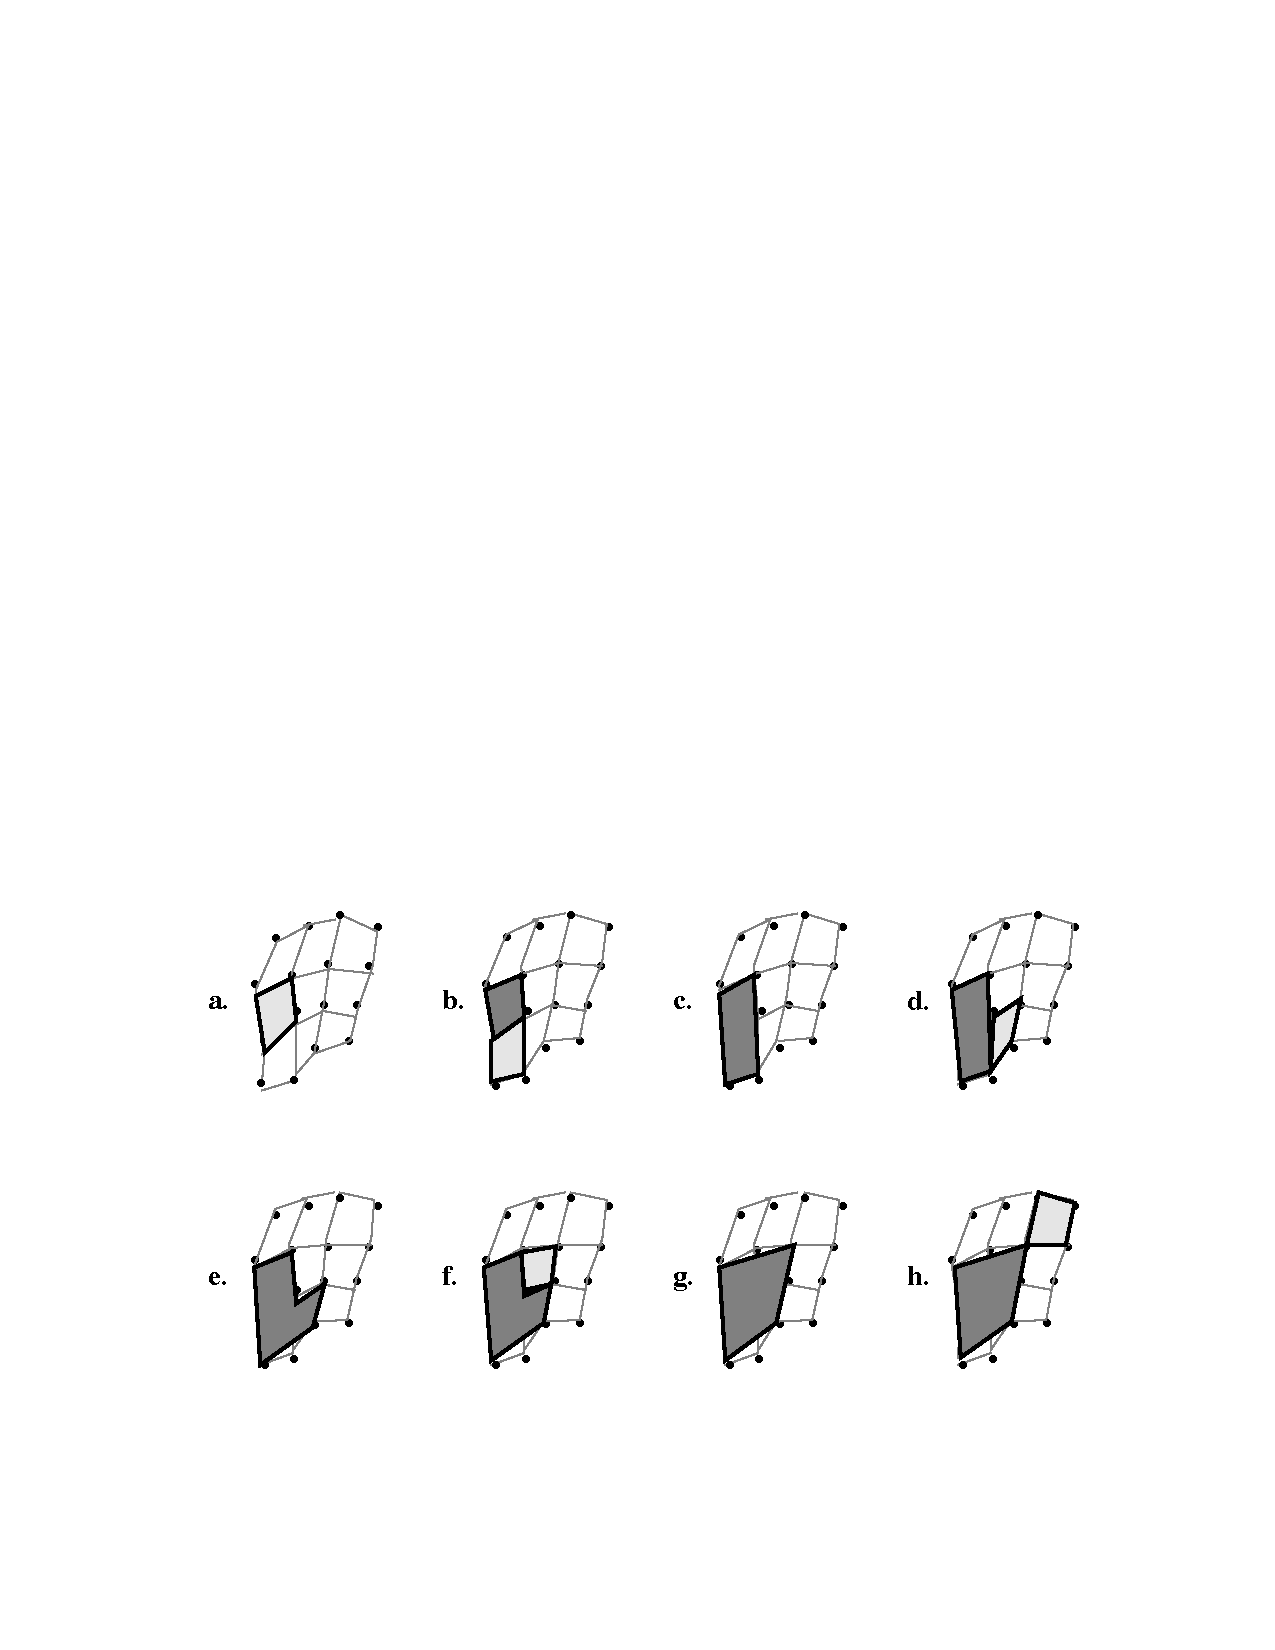
\includegraphics[width=12cm]{chapter10/polygonGrowth.pdf}
%\caption[Polygon growth]{Polygon growth. Image courtesy of \cite{Dehaemer91}.}
%\label{chap10:fig-polygonGrowth}
%\end{figure}
%
%This method of fitting polygons to the sampled data is not as useful as the adaptive subdivision methods, for several reasons. First, it is an essentially brute force method of surface fitting and very repetitive in nature. Many trial polygons are created, only to be 'thrown out' because they exceed the error tolerance. This causes the procedure to execute quite slowly (orders of magnitude more slowly) than the adaptive subdivision method. Second, the data is not significantly reduced. Many of the generated polygons are of complicated shapes and use a large number of vertices. Thus many of the original sample data points are retained.
%
%
%\subsubsection*{Appearence preserving simplification.}
%A completely different approach to determining the error associated with a given simplification operation was described by \cite{Cohen98}. Their metric, which is appearance-based, measures the amount of deviation caused by the operation in the screen-space (pixelised) representation of the mesh. Their algorithm functions by decoupling surface position from color and curvature information and storing the latter two quantities in texture and normal maps. A traditional geometric simplification algorithm can then be employed to filter the surface position, while a hardware-based approach is used to filter the color and normal information, resulting in simplified representations that are nearly visually indistinguishable from the original. However, the algorithm requires a parameterisation of the mesh in order to function.
%
%
%\subsection{Global simplification strategies}
%
%\subsubsection*{Vertex clustering.}
%The method of vertex clustering was originally proposed by \cite{Rossignac93} to handle meshes of arbitrary topological structure. In their algorithm, each vertex in the input mesh is assigned a weight based on its perceptual importance: vertices adjacent to triangles with large faces and those in areas of high curvature are weighted more heavily than vertices in smooth regions adjacent to smaller triangles. Next, a bounding box is placed around the mesh and subdivided into a three-dimensional grid. Finally, all the vertices in a given grid cell are clustered to the position of the vertex with maximum weight. Degenerate geometry may then be removed, although the authors proposed a novel visualisation of certain degenerate faces and edges in an effort to enhance the recognizability of their simplified meshes. The algorithm is extremely efficient and simple to implement, and the level of simplification may be controlled (although with some difficulty) by choosing the resolution of the overlaid grid. However, vertex clustering can drastically alter the topology of the input mesh in an unpredictable manner, and in practice does not produce very faithful geometric approximations at low levels of detail.
%
%\subsubsection*{Re-tiling.}
%The re-tiling method described by \cite{Turk92} begins with a polygonal surface and creates a triangulation of this surface with a user-specified number of vertices. The points are placed uniformly over a given polygonal surface by distributing points at random over the surface and then having each point repel all of its neighbors. An alternative to placing the points randomly is using the variation in surface curvature. The features of the surface would be more accurately reflected in a re-tiling by increasing the density of vertices in regions of high curvature.
%
%The key notion in the re-tiling procedure is the creation of an intermediate model called the mutual tessellation of a surface that contains both the vertices from the original model and the new points that are to become vertices in the re-tiled surface. The new model is then created by removing each original vertex and locally re-triangulating the surface in a way that matches the local connectedness of the initial surface (see \fig{chap10:fig-retiling}).
%
%If this method produces nice meshes, an issue is finding measures of how closely matched a given re-tiling is to the original model. 
%%
%\begin{figure}
%\centering
%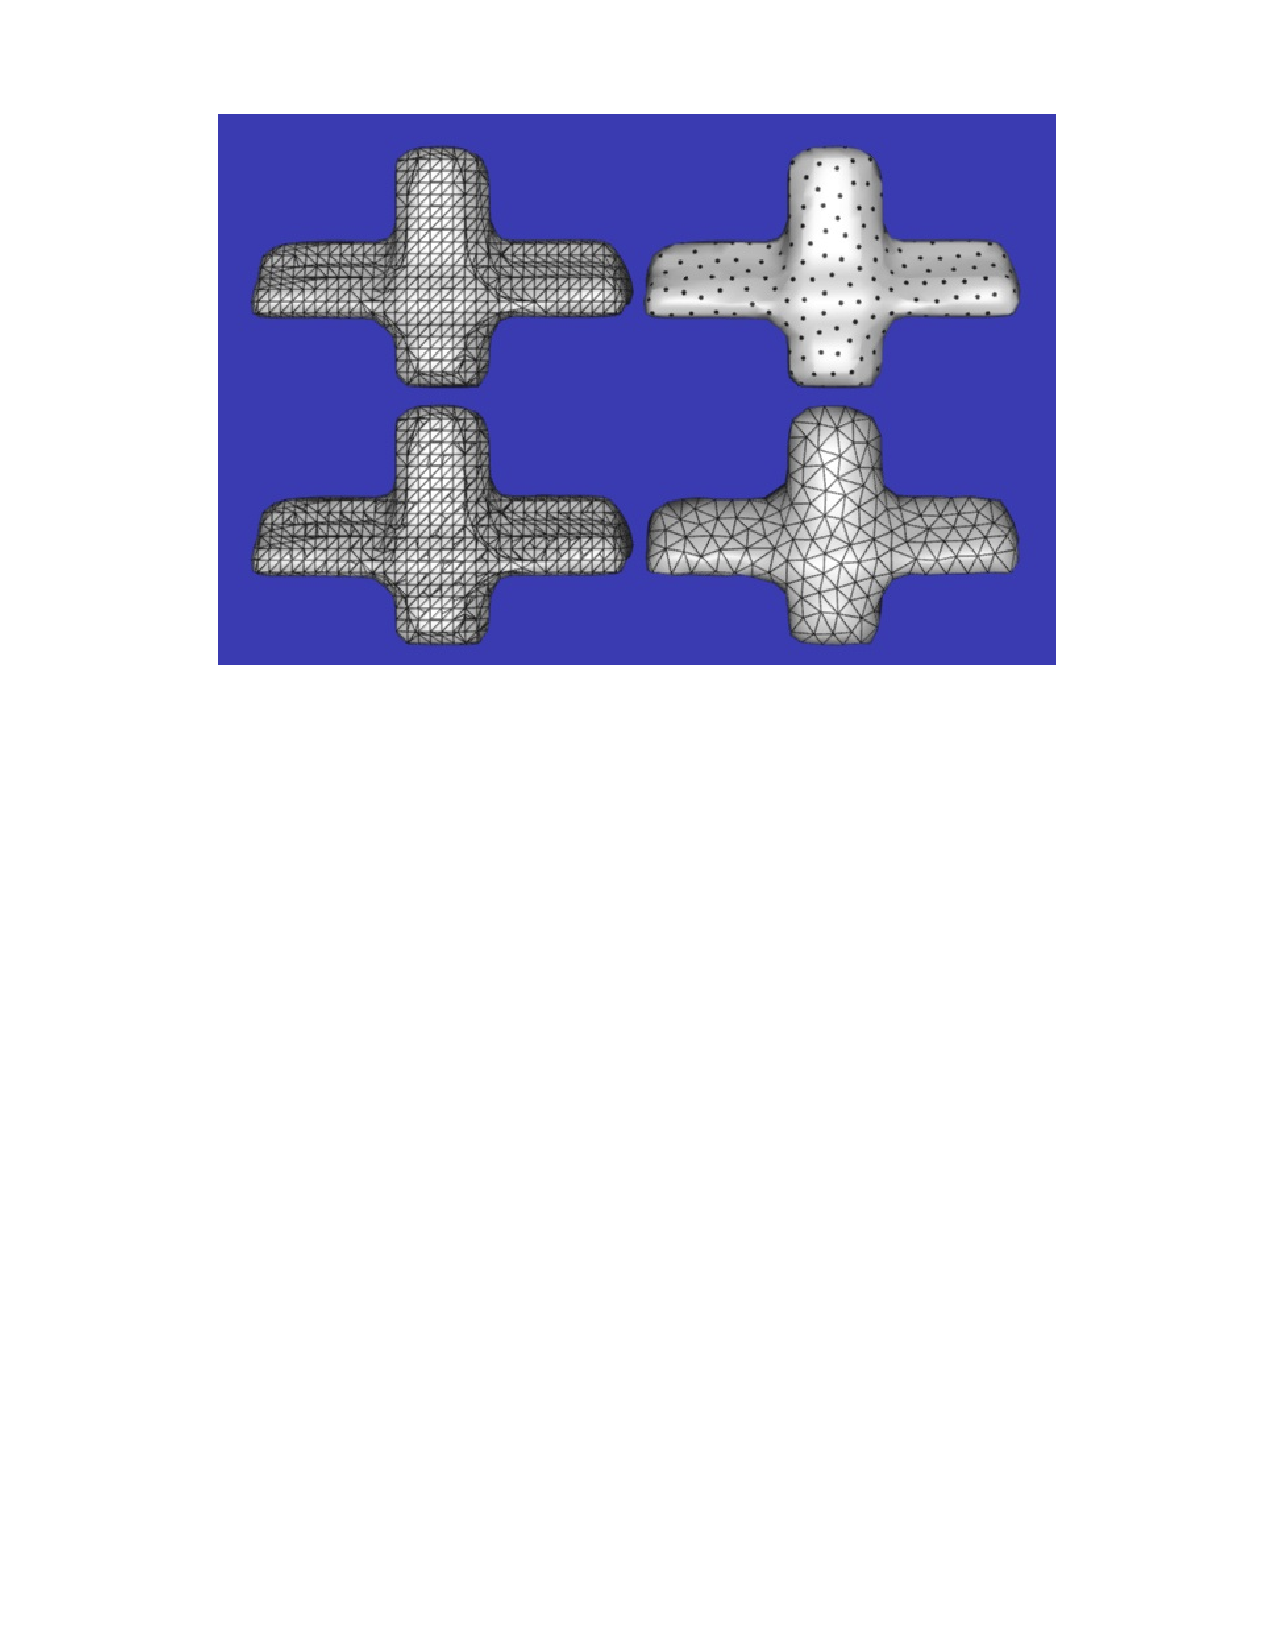
\includegraphics[width=12cm]{chapter10/retiling.pdf}
%\caption[Retiling technique]{Upper left: original surface. Upper right: candidate vertices after point-repulsion. Lower left: mutual tesselation. Lower right: final tesselation. Image courtesy of \cite{Turk92}.}
%\label{chap10:fig-retiling}
%\end{figure}


\section{Our method}

	\subsection{A simple algorithm}
	
In the following, we assume that we have a high resolution triangular mesh obtained from a binary segmented image of the object we want to simulate (via a Marching Cube algorithm for instance, \cite{Lorensen87}). We propose a technique that can simplify the high resolution mesh of the object to be simulated and approximate the surface of anatomical structures with shell elements whose each surface is described by the shape function used in our shell formulation. Thus, the first step in the process of generating a shell-based mesh is an important decimation of the high resolution mesh, using quadric edge collapse technique implemented in \citeauthor{Meshlab}. MeshLab is an open source program for the processing and editing of unstructured 3D triangular meshes. The algorithm tries as much as possible to preserve mesh boundaries and generates high quality triangular elements. We then apply a heuristic method derived from the work of \cite{Saupin07} with tetrahedral meshes based on simple geometrical rules. For each node of the coarse mesh, we find the three closest triangles on the high resolution mesh and we move the node to the barycentre of the three centres of mass of those triangles. This technique locally smoothes the surface of the mesh while converging towards the desired high resolution mesh. 

At each iteration of this algorithm, we want to measure the error between the curved surface of shells and the target. Indeed, we need to ensure that the distance between the surface of our shell-based mesh and the targeted high resolution mesh will be minimal. An efficient technique for measuring the error between two surfaces is the Hausdorff distance \citep{Klein96}. As a reminder the Hausdorff distance between two meshes is the maximum between the two so-called one-sided Hausdorff distances:
\begin{equation}
d_{\mathrm{H}}(X,Y) = \max \left\{ \sup_{x \in X} \inf_{y \in Y} d(x,y), \sup_{y \in Y} \inf_{x \in X} d(x,y) \right\},
\end{equation}
where $d()$ is the Euclidian distance between two points. The same technique of subdivision used for rendering allows us to sample the actual surface described by the shells to compute the Hausdorff distance with the targeted high resolution mesh. 

By using the Hausdorff distance between two iterations, the process may be stopped when the required precision has been reached. A simple example is shown \fig{chap10:fig-cylinder} to illustrate the method. 
\begin{figure}[ht]
\centering
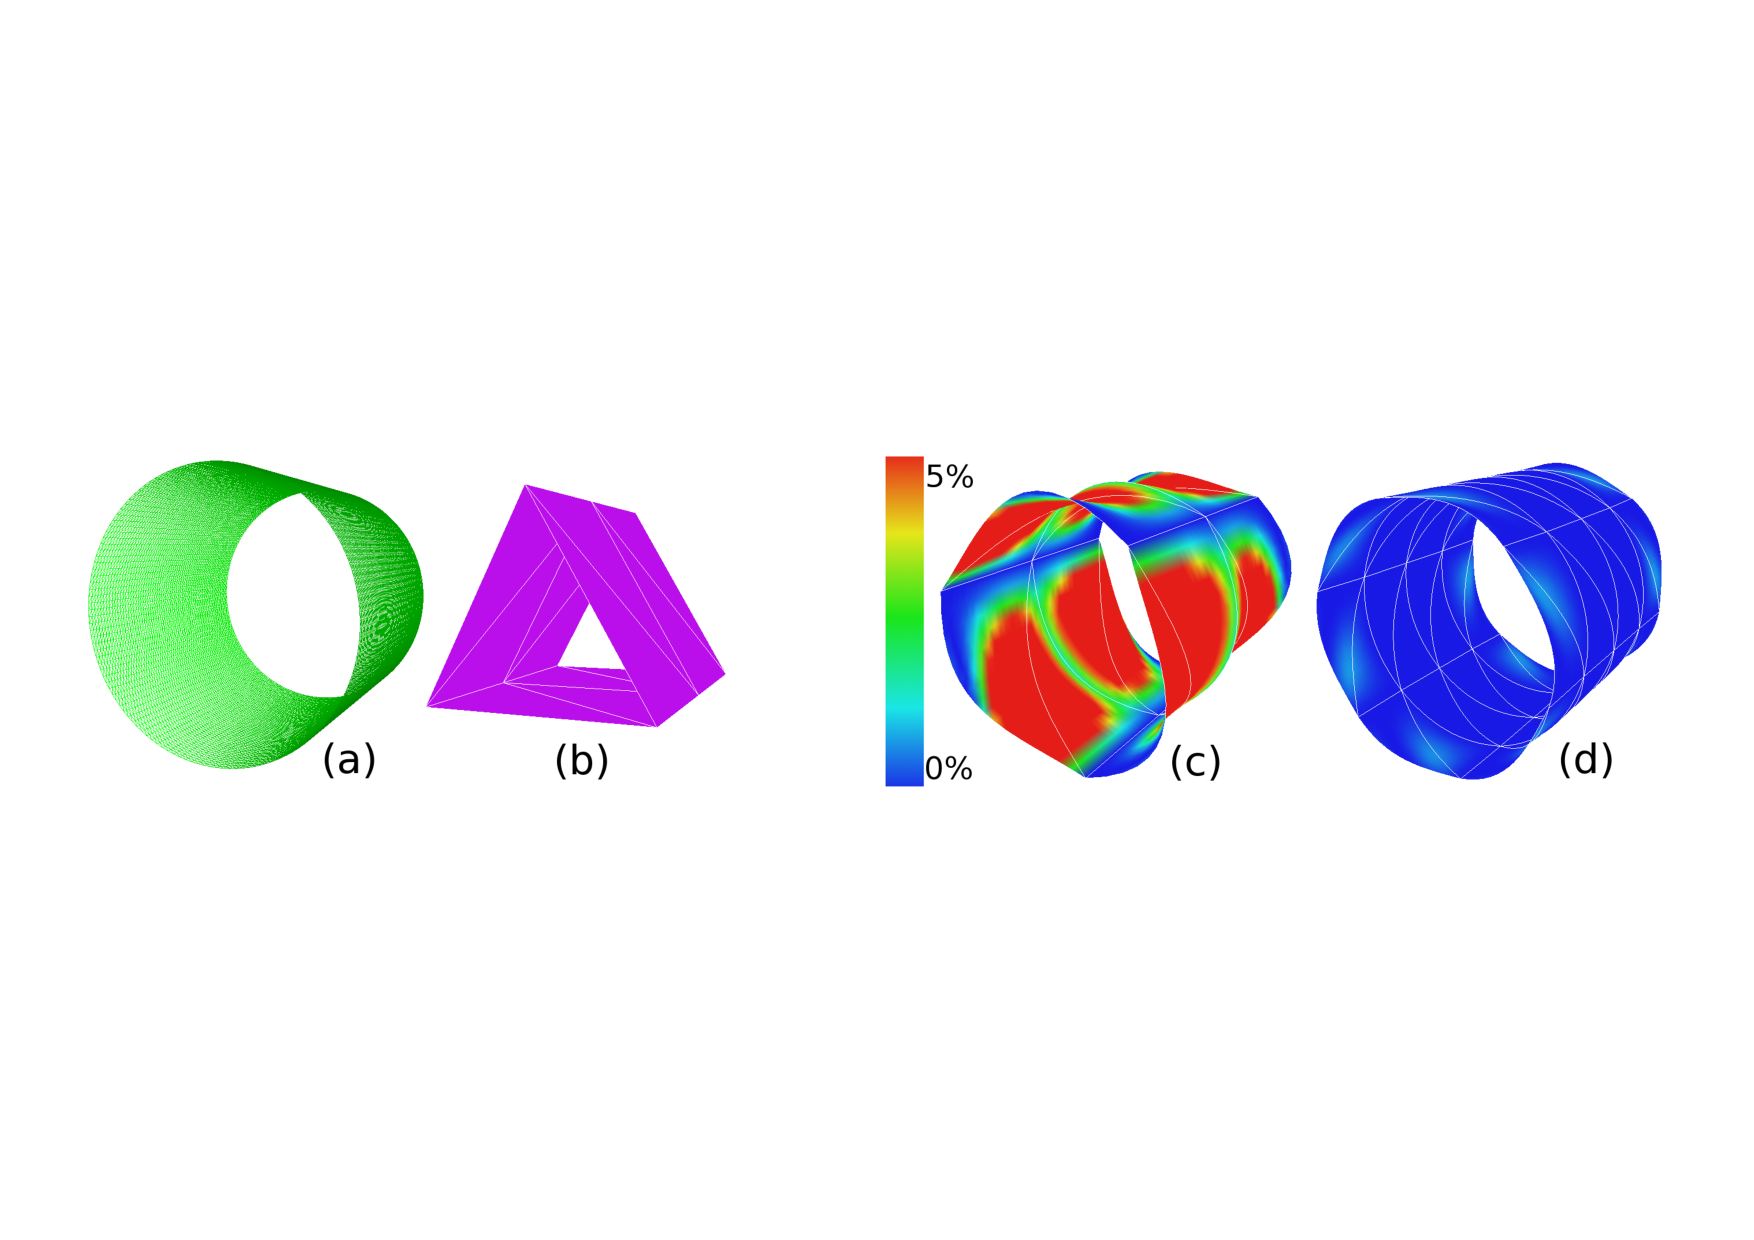
\includegraphics[width=13.5cm]{chapter10/exampleCylinder.pdf}
\caption {The target (a) is a high resolution cylinder mesh of 16,384 triangles and we start from a very coarse mesh (12 triangles), rendered with flat triangles here (b). In (c) the coarse mesh is rendered with shells and a one-sided Hausdorff distance colour map is applied to show the initial error with the high resolution mesh. (d) One-sided Hausdorff distance colour map after one iteration of our algorithm (48 shells).}
\label{chap10:fig-cylinder}
\end{figure}

	\subsection{Results on complex anatomical structures}
	
\subsubsection*{Meshing of anatomical structures.}
This approach has been applied to approximate more complex anatomical geometries with curved shell elements. Two examples are given with the Glisson's capsule, which is the membrane surrounding the liver (\fig{chap10:fig-liver}) and an aneurysm (\fig{chap10:fig-aneurysm}). In each case, the error is computed through a Hausdorff distance and expressed as a percentage of the diagonal of the object's bounding box. 
%
\begin{figure}[ht]
\centering
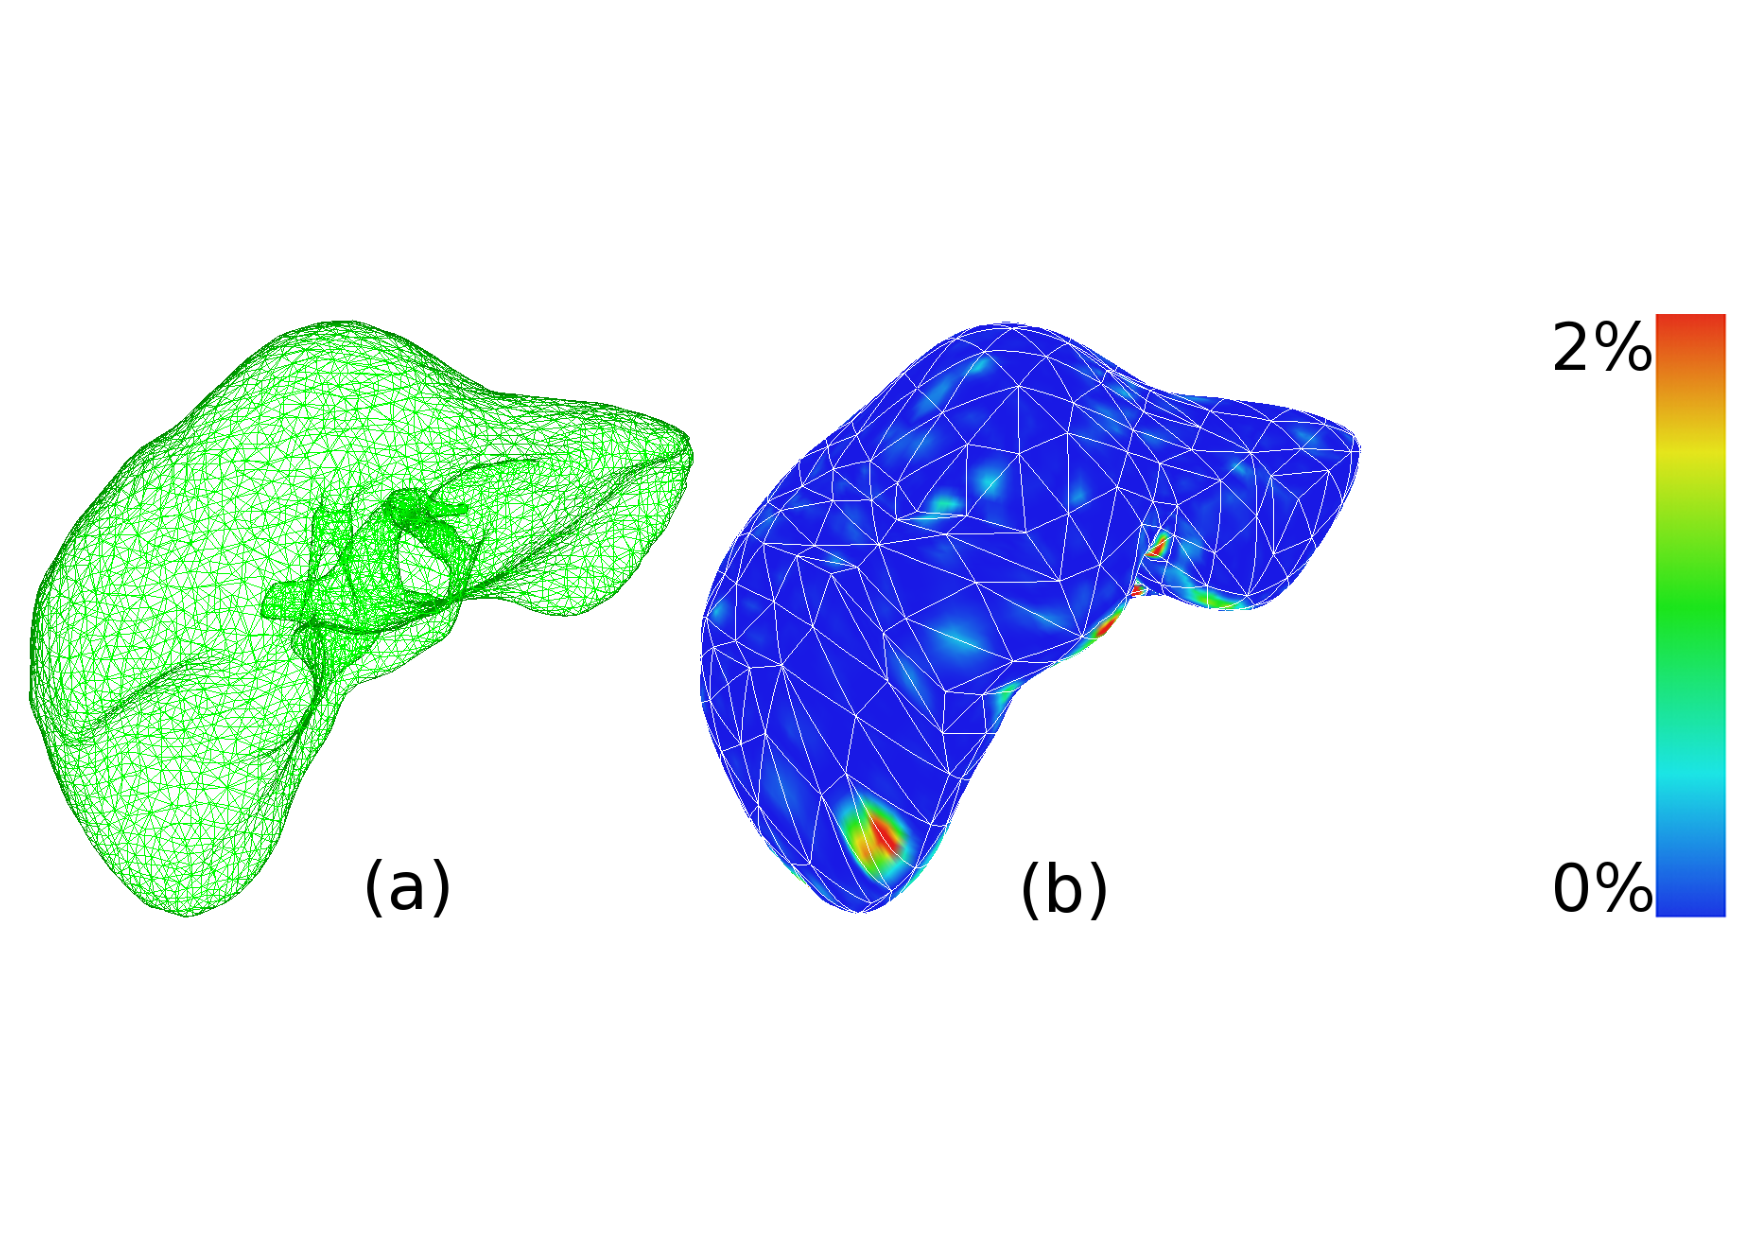
\includegraphics[width=13.5cm]{chapter10/resultsLiver.pdf}
\caption {(a) the targeteted high resolution Glisson's capsule mesh ($8\,000$ triangles). (b) the one-sided Hausdorff distance error map after applying only one iteration of our algorithm to the coarse mesh ($1\,200$ shells).} 
\label{chap10:fig-liver}
\end{figure}

\begin{figure}[ht]
\centering
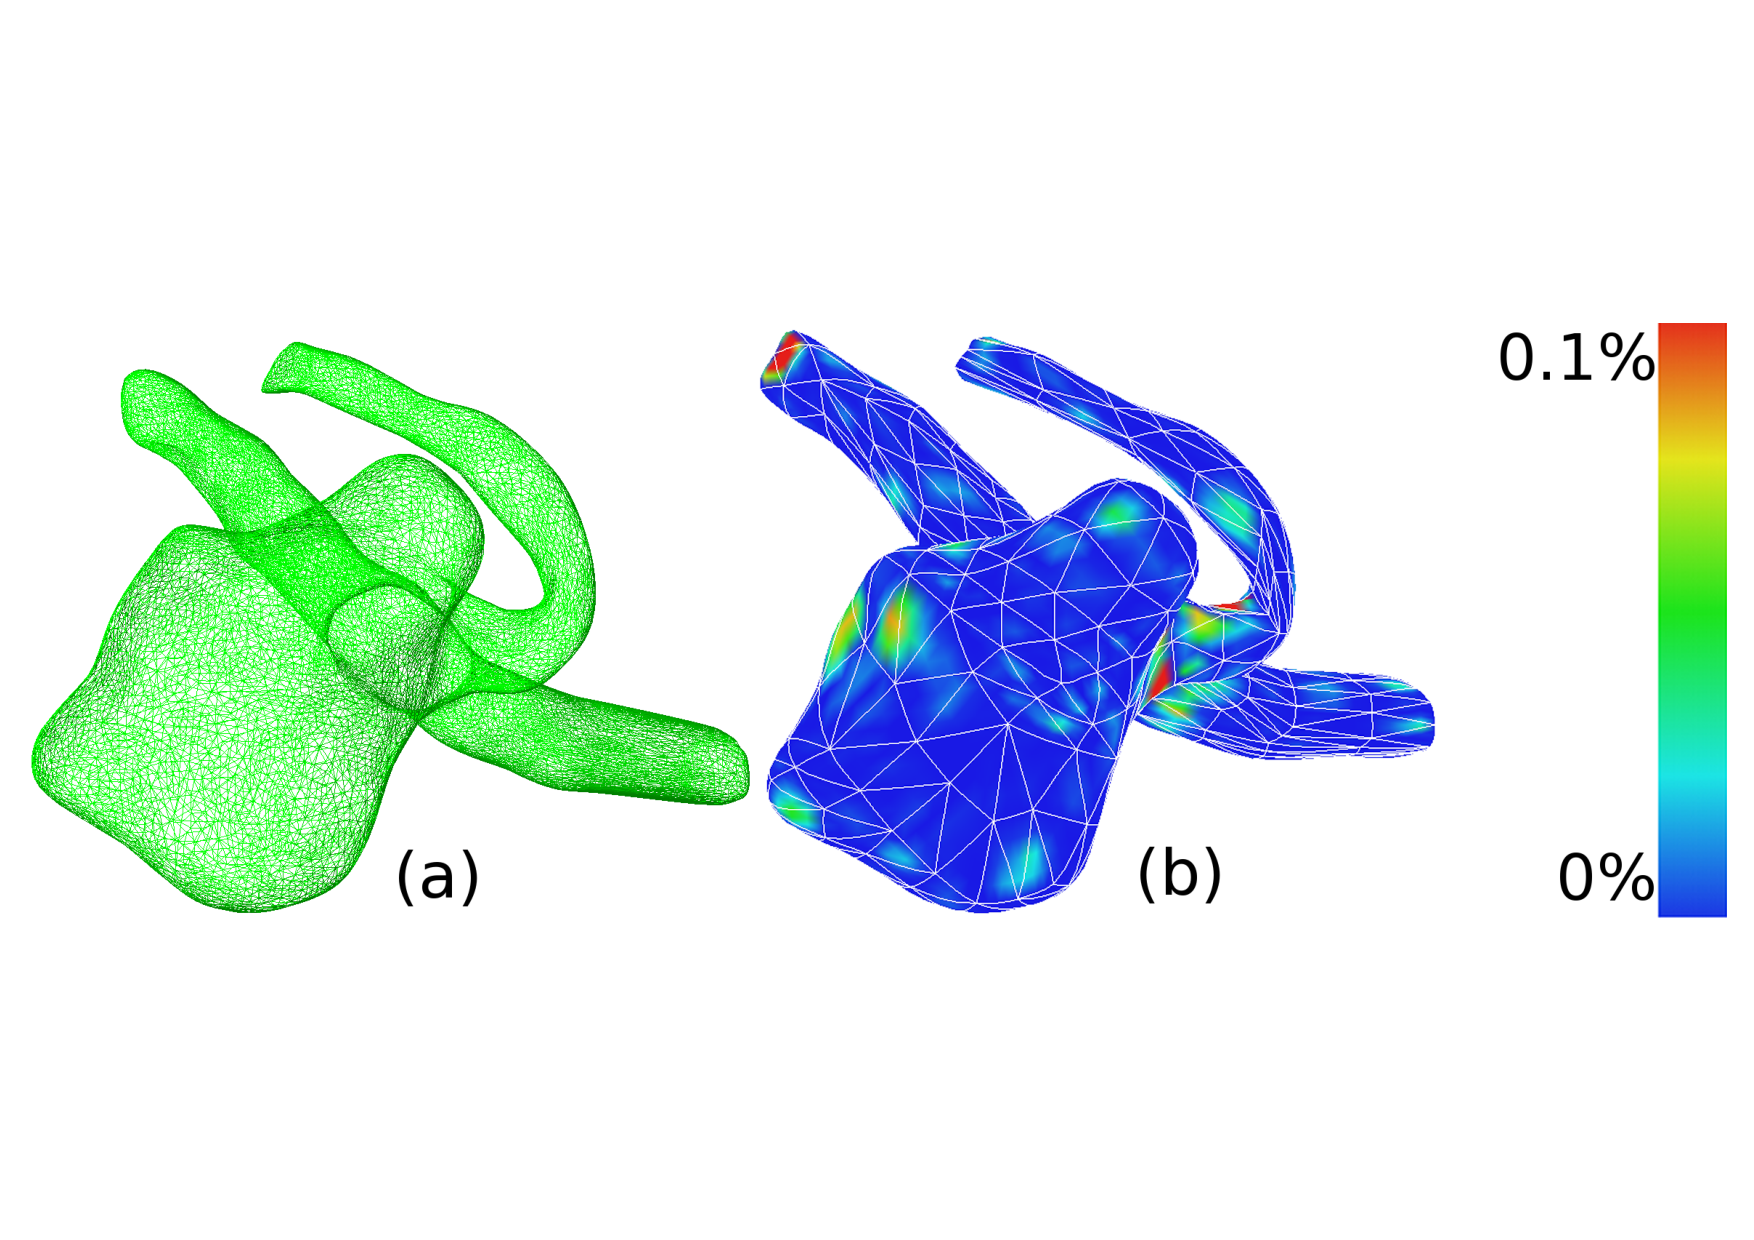
\includegraphics[width=13.5cm]{chapter10/resultsAneurysm.pdf}
\caption {(a) the targeteted high resolution aneurysm mesh ($28\,368$ triangles). (b): the one-sided Hausdorff distance error map on a mesh of 772 shells generated with our method.}
\label{chap10:fig-aneurysm}
\end{figure}

\subsubsection*{Computation times.}
We perform several tests on the aneurysm model at different resolutions to measure computation times. The shells are resisting to a uniform pressure load and solved using a Conjugate Gradient (CG) iterative solver. The computation times are reported in \fig{chap10:fig-computation}. Implicit integration allows for large time steps ($40\,ms$) and the computation is real-time for 800 shell elements and a reasonable error criterion ($5\,\%$). When the computation time must be bounded (critical real-time applications), one can fix the number of CG iterations to, for instance, $100$ and remains real-time for $1\,000$ shell elements. However, in that case the accuracy of the results is not checked.
%
\begin{figure}[ht]
\centering
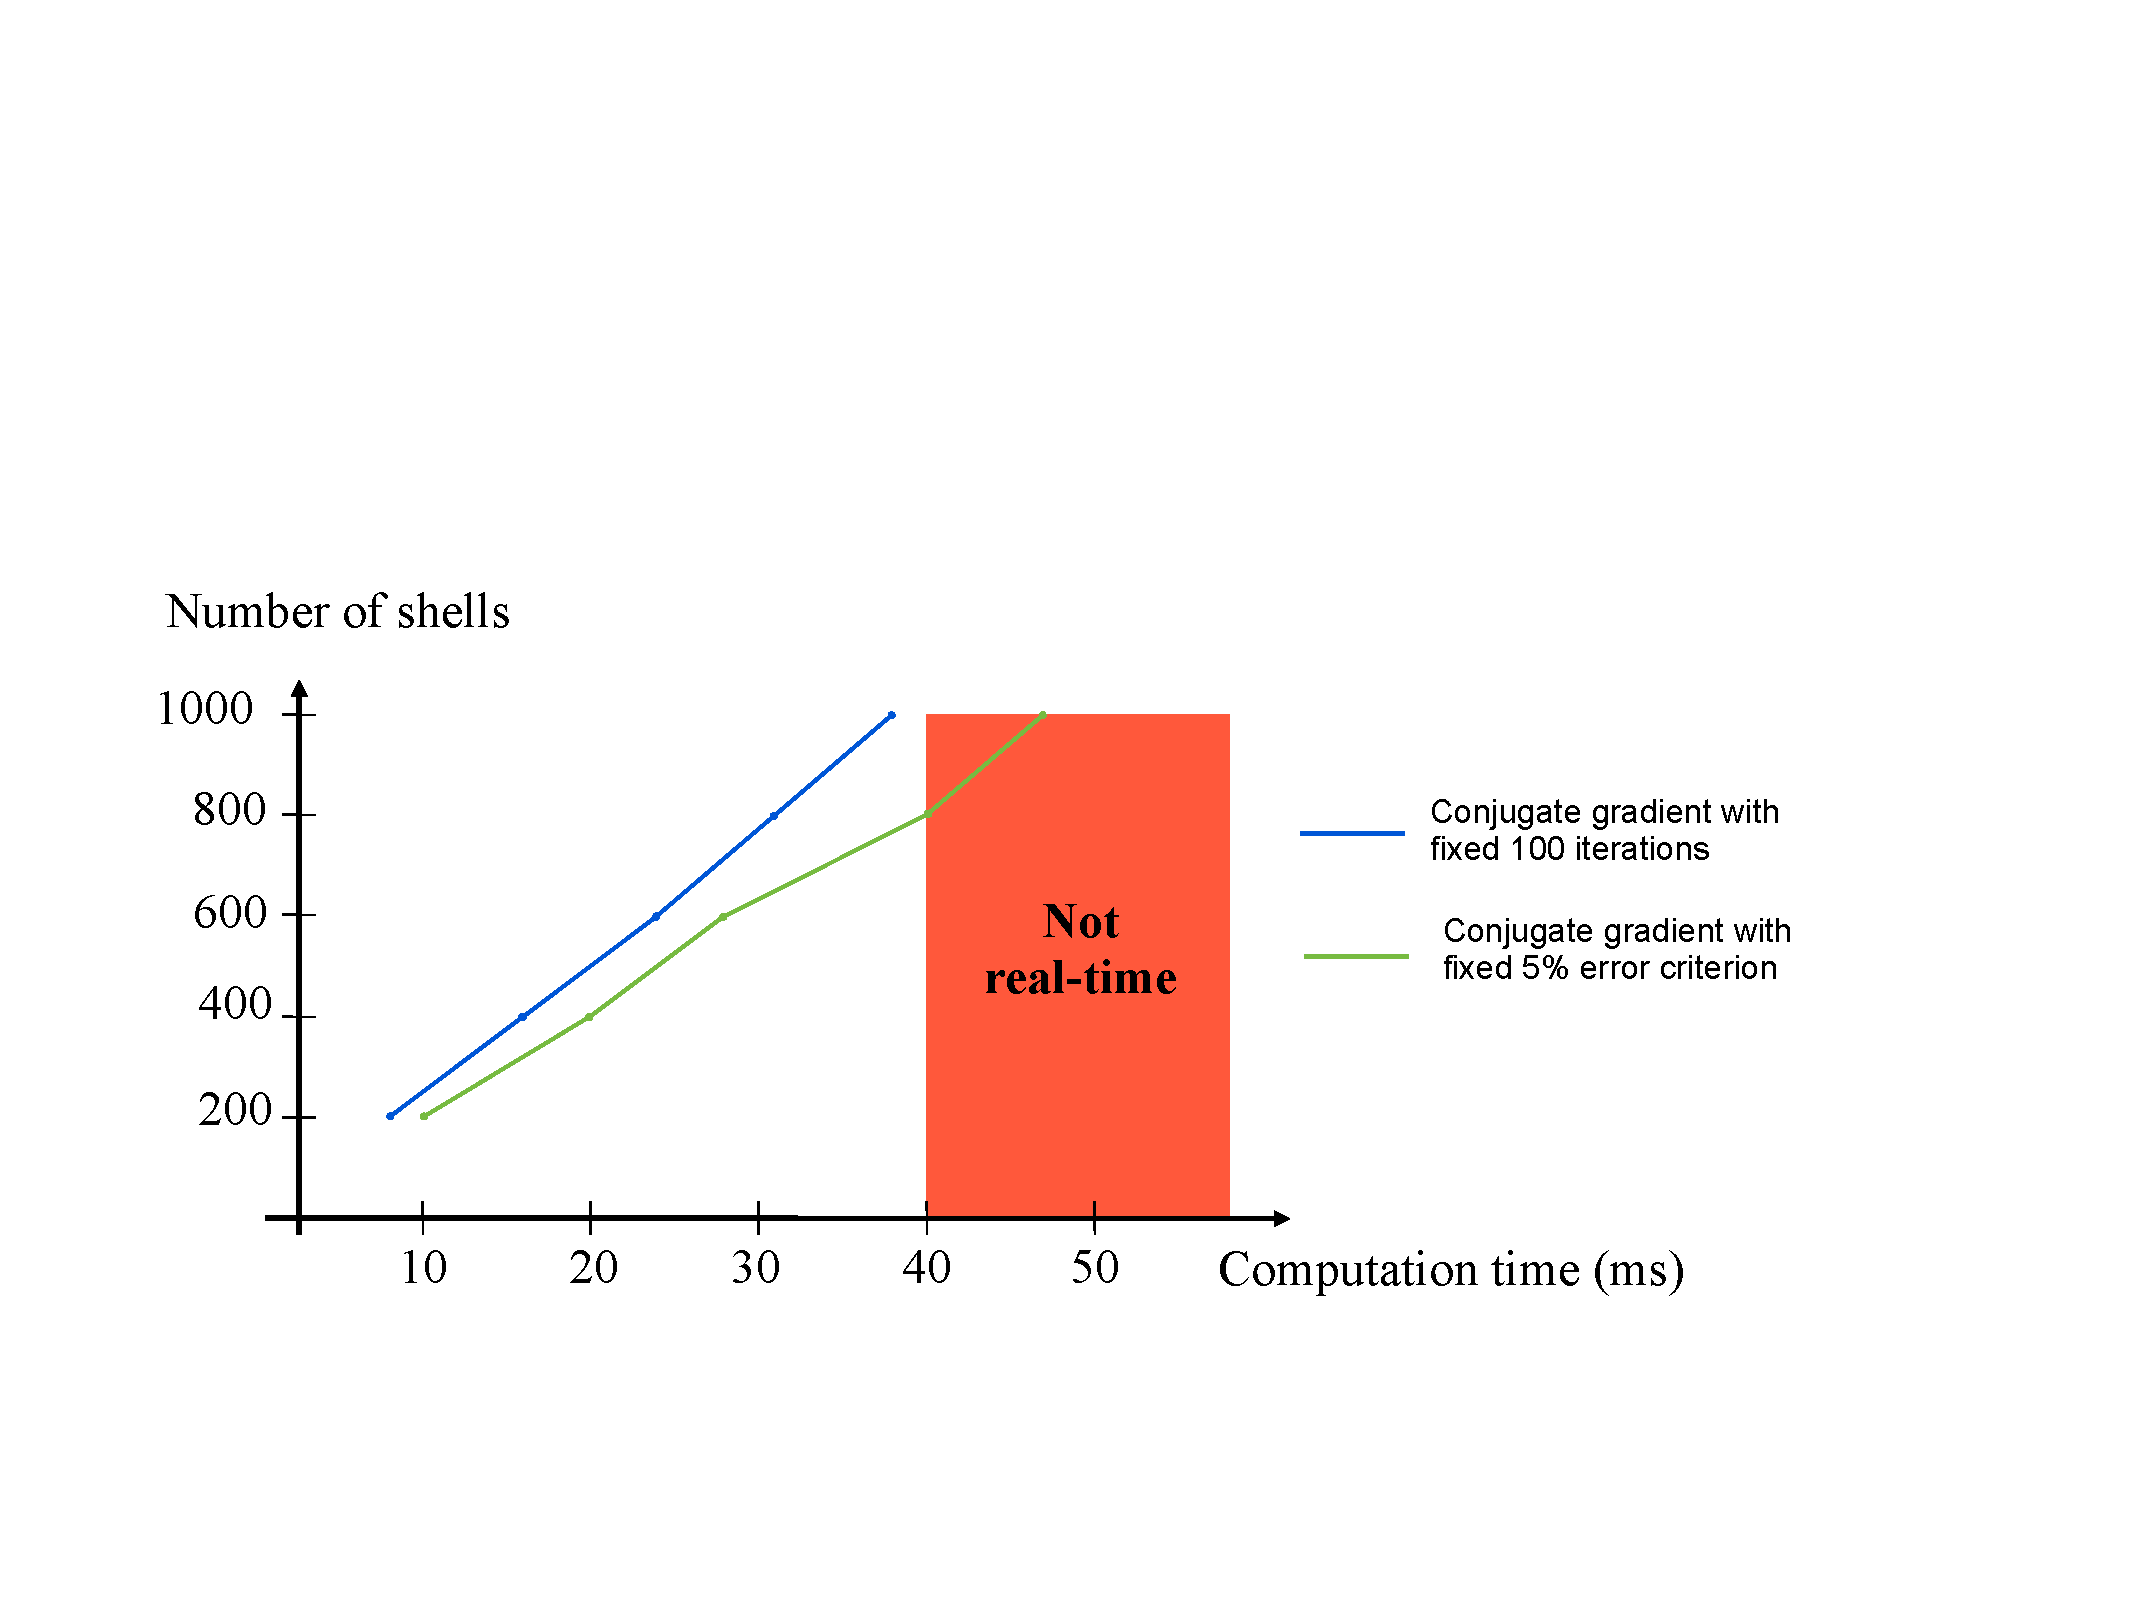
\includegraphics[width=13.5cm]{chapter10/computation_times.pdf}
\caption {Computation time on meshes of 200, 400, 600, 800 and $ 1\,000 $ elements.}.
\label{chap10:fig-computation}
\end{figure}

\subsection{Coupling between tetrahedra and shells for advanced modelling}
Structures in human body can be either solid (brain, liver, prostate etc.) or hollow (colon, blood vessels, stomach etc.). However, knowing how to model the two kind of structures is not sufficient to reach a high degree of accuracy, real life situations are more complex. As an example, the external surface of the liver is covered by a layer of cells called Glisson's capsule. Its interaction with the liver plays an important role into the overall structure's mechanical behaviour. Therefore considering the interaction between solid and hollow objects is as crucial as modelling the two structures separately. 

An example of medical procedure to illustrate this point even further is angioplasty. Angioplasty is the technique of mechanically widening a narrowed or obstructed blood vessel, typically as a result of atherosclerosis. An empty and collapsed balloon on a guide wire is passed into the narrowed locations and then inflated to a fixed size. The balloon crushes the fatty deposits, so opening up the blood vessel to improved flow. As a proof of concept, we tried to simulate an angioplasty. Our preliminarty results are presented on \fig{chap10:fig-stent}. The blood vessel is modelled using the shell FEM formulation described in this paper and the fatty deposits are simulated with a tetrahedral FEM method and are fixed to the interior wall of the blood vessel. When the balloon inflates it crushes the deposits and they then apply a pressure onto the curved surfaces of shells modelling the interior wall. The forces are then distributed onto the mechanical nodes of the blood vessel mesh as detailed in section~\ref{chap9:interactions}, which widens the blood vessel as expected. 
%
\begin{figure}[ht]
\centering
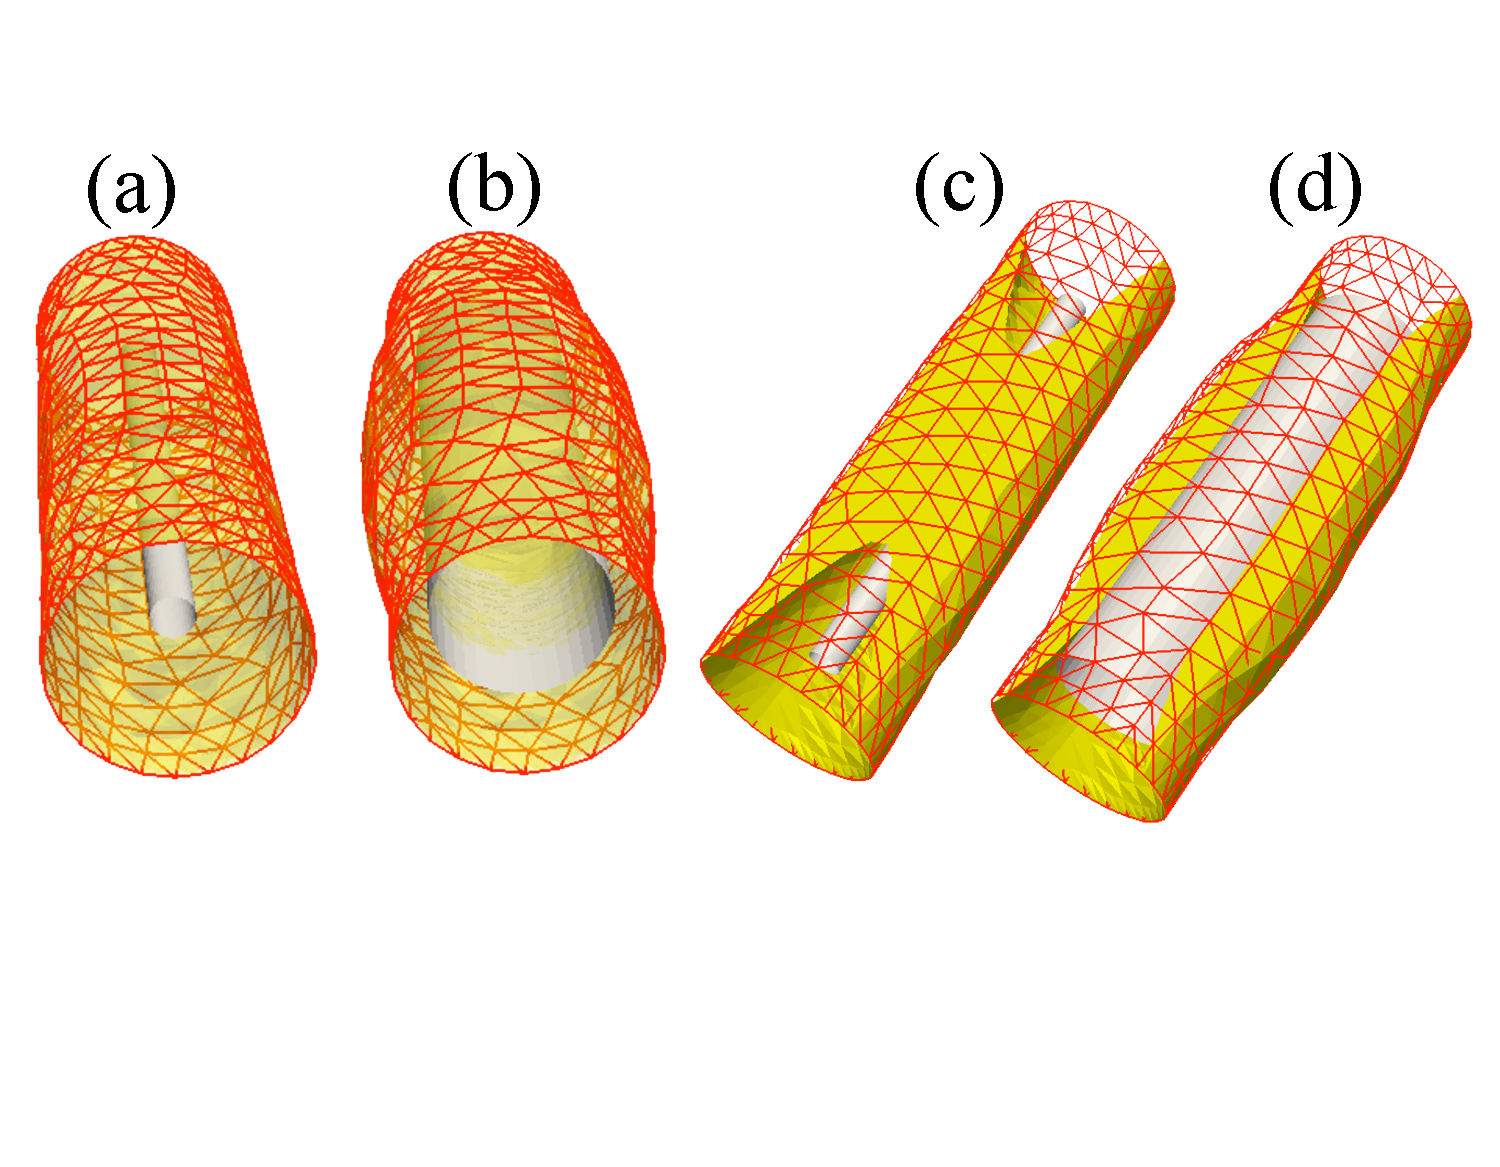
\includegraphics[width=12cm]{chapter10/stenose_final.pdf}
\caption {Simulation of an angioplasty procedure. (a, c): A collapsed stent is inserted into the blood vessel simulated with our shell FEM formulation. The fatty deposits (in yellow) are modelled with tetrahedral FEM. (b, d): The stent is crushing the fatty deposits which creates a pressure onto the interior wall and widens the blood vessel.}
\label{chap10:fig-stent}
\end{figure}

\section{Discussion}

We proposed a framework for real-time modelling of thin anatomical structures. The novelty of our method relies on the combination of a shell finite element formulation and a geometric surface reconstruction both based on the same polynomial interpolation function used to describe the surface of shells. We also show how contacts and interactions with the curved surfaces of shells can be handled using the same function. In summary, these polynomial shape functions are used in three different ways in our computational model:
%
\begin{description}
\item[(a)] to approximate complex geometrical shapes
\item[(b)] to compute internal forces via a co-rotational shell FEM
\item[(c)] to compute contact forces onto a curved triangle
\end{description}

We achieved our objectives to propose a versatile solution which can simulate, in real-time, thin objects with various shapes and material properties with good accuracy. The efficiency of the method was illustrated through shell-based reconstruction and real-time simulation of the deformations of various anatomical structures and other thin objects (like an intra-ocular implant). We also presented preliminary results on the coupling between solid (tetrahedra) and thin objects (shells) for the advanced modelling of anatomical structures via the simulation of an angioplasty procedure. 

\bigskip

The finite element procedure that we propose is largely developed based on physical understanding without the use of mathematical shell theories. Indeed, our shell FEM was obtained by simply superimposing a plane stress and bending energies. According to \cite{Chapelle03}, this type of approach has a limited level of accuracy. The effective study of shell structures clearly requires a deep physical understanding of shell structural behaviours. The complexity of the physical behaviours of shells requires advanced mathematical analyses from theories that are still in development. The interested reader may refer to the book of \cite{Chapelle03} for more details on shell theory. If the range of application of our shell formulation might be somewhat limited, we did not find out any inconsistencies through our tests. We also need to keep in mind that the accuracy required in medical simulation is not the same than the one demanded in structural analyses for instance. Moreover, the additional complexity of a shell finite element formulation based on true shell theory may also very well jeopardise our real-time constraints. Therefore, we do not think that the use of this simple shell formulation significantly diminishes our contribution to the field of medical simulation. Indeed, to our knowledge, our co-rotational shell FEM is the first description of a shell finite element model applied to simulating the deformation of thin anatomical structures. 

Nevertheless, a few improvements are conceivable. Large strain could be allowed by using a non-linear strain tensor and more complex material laws (non-linear, viscoelasticity, etc.) could also be added to our shell formulation. However, those changes are substantial and their implementations are not straightforward. In addition, it is not clear how the benefits would be the greatest: whether from enhancing our model to a non-linear formulation or completely changing to another model based on true shell theory (where membrane and bending energies are not separated). The answer may depend on the type of constraints applied on the object. Also (as already mentioned section \ref{chap9:GPU}), the real-time capacity of our algorithm could be further improved by implementing our shell FEM on GPU. Although an optimal parallel re-implementation is always challenging, we have already reviewed why there was no major obstacle to a GPU implementation. 

Although we were able to mesh complex anatomical structures with a fairly small number of shell elements, our approach suffers from two major drawbacks. In our current implementation, if the error measured with the Hausdorff distance is greater than a threshold (which is also difficult to choose), all triangular elements are subdivised into 4 new triangles and each of the new vertices is moved towards the targeted geometry based on our heuristic algorithm. Obviously, this is not optimal as the error between the two meshes may very well be local and therefore the use of a global mesh refinement may be very limited. The second drawbrack is that we also do not check the quality of the elements during our mesh process. If some elements are stretched from the heavy decimation, these elements are not corrected during the process of remeshing. Our algorithm could even worsen the situation by splitting those stretched elements into four smaller (and more stretched) elements. One solution for the latter issue would be to enhance our algorithm with a relaxation phase where a repulsion force is applied between each vertex (constrained to remain on the surface of the object). This physical approach would allow a more even distribution of the vertices across the surface and would contribute to obtain better quality elements overall. Yet, meshing a surface with curved elements is a very complex problem and still an active area of research. In contrast to all previous geometrical techniques, we suggested a more physical approach consistent with our shell FEM formulation and obtained good results in meshing complex anatomical structures. 
